\subsection{ToN-IoT}

\subsubsection{Descripción}

ToN es un dataset creado por la University of New South Wales Canberra, Australia \cite{9189760}. Para generarlo, se estructuró un entorno de red con tres capas llamadas Edge, Fog y Cloud para simular un entorno realista. Como tecnología de virtualización, se utiliza NSX-VMware, el cual permite definir una red a través de software (SDN), y para gestionar las máquinas virtuales se ha hecho uso de VMware vSphere hypervisor NFV.

Para la capa Edge, tenemos diferentes dispositivos físicos, un servidor NSX VMWare y diferentes equipos de red. En esta capa, se incluyen diversos sensores IoT tanto simulados como reales y comunicados a través de MQTT. Adicionalmente, se incluyen hosts de usuarios como teléfonos móviles y un televisor. En esta capa, los dispositivos se les asigna una dirección IP en el rango 192.168.1.0/24 a través de DHCP.

En la capa Fog tenemos diferentes máquinas virtualizadas, incluyendo dispositivos vulnerables, atacantes y middleware. Estos son:
\begin{enumerate}
  \item Diez máquinas atacantes con Kali Linux (192.168.1.30-39) con diferentes scripts de ataque.
  \item Máquina virtual ofreciendo DVWA, una aplicación web vulnerable (192.168.1.192)
  \item Máquina virtual con Metasploitable3, una distribución Linux específicamente diseñada para ser vulnerable contra la cual hacer pruebas. (192.168.1.194)
  \item Máquina virtual con OWASP Security Shepherd, una plataforma conteniendo aplicaciones vulnerables sobre las cuales hacer pruebas (192.168.1.184)
  \item Servidor Ubuntu ofreciendo diferentes servicios con FTP, HTTPS, etc. (192.168.1.190)
  \item Un servidor para registrar registros de red de todos los servicios activos (192.168.1.180)
  \item Máquina virtual con Windows 7 (192.168.1.193)
  \item Máquina virtual con Windows 10 (192.168.1.195)
\end{enumerate}

La capa Cloud contiene varios servicios como un broker MQTT, una web vulnerable en PHP, entre servicios cloud para gestionar los mensajes. Esta capa recibe los datos de los dispositivos IoT para ser procesados.

Los dispositivos IoT utilizados consisten en una nevera inteligente, una puerta de garaje remotamente controlada, un objeto con GPS, luces activadas por movimiento, un servicio Modbus con el que se comunican diferentes valores de registros, un termostato inteligente y un sistema de monitorización del clima.

Aparte del tráfico benigno, hay 8 ataques, los cuales se han realizado en el momento de generar datos. Estos consisten en:
\begin{enumerate}
  \item \textbf{Escaneo}: ataque basado en el escaneo de puertos para descubrir vectores de ataque potenciales. Se han utilizado nmap y nesus para escanear los puertos disponibles en los dispositivos IoT víctima en el rango 192.\-168.\-1.\-0/24 y en el broker MQTT. Las IP de los atacantes consisten en 192.\-168.\-1.\-30, 192.\-168.\-1.\-31, 192.\-168.\-1.\-32, 192.168.1.\-33 y 192.168.1.\-38
  \item \textbf{Denegación de servicio}: ataque basado en saturar los recursos de un dispositivo para denegar el servicio legítimo. A través de scripts de Python y UFONet se ha tratado de generar ataques de denegación de servicio (dsitribuidos y no distribuidos). Las IP de los atacantes en los ataques no distribuidos son 192.\-168.\-1.\-30, 192.\-168.\-1.\-31 y 192.\-168.1.\-39. Los distribuidos se han realizado desde 192.\-168.\-1.\-30, 192.\-168.\-1.\-31 y 192.\-168.\-1.\-(34-38)
  \item \textbf{Ransomware}: ataque basado en encriptar el sistema de ficheros y vender las claves de descifrado por un precio, 'secuestrando' el sistema. El ataque se ha realizado a través del sistema con Metasploitable3 y las IP de los atacantes son 192.168.1.33 y 192.168.1.37.
  \item \textbf{Puertas traseras}: ataque basado en generar en un sistema la capacidad de obtener acceso remoto no autorizado. Se ha utilizado Metasplotaible3 y los ataques se han generado desde 192.168.33 y 192.168.1.37
  \item \textbf{Inyección}: ataque basado en inyectar datos maliciosos para manipular comandos de control e interrumpir el funcionamiento normal del sistema. Se han utilizado scripts en Bash para realizar la inyección y han participado los sistemas 192.168.1(30, 31, 33, 35, 36, 38).
  \item \textbf{Cross-Site Scripting}: ataque basado en provocar la ejecución de código arbitrario en el navegador saltándose las barreras de seguridad entre dos páginas web. Se han utilizado scripts en Bash y la herramienta XSSer para generarlo desde 192.168.1.(32, 35, 36, 39).
  \item \textbf{Descifrado de contraseñas}: ataque basado en fuerza bruta y/o diccionarios para descubrir las claves de acceso a dispositivos. Se han utilizado dos scripts con las herramientas CeWL y Hydra para los ataques de diccionario y fuerza bruta, respectivamente. Los dispositivos atacantes consisten en 192.168.1.(30, 31, 33, 35, 38).
  \item \textbf{Man-In-The-Middle}: ataque basado en tratar de interponerse en medio de las comunicaciones entre dos dispositivos para interceptar información y potencialmente modificar los datos. Los ataques generados se han basado en el envenenamiento del cache ARP, redirección ICMP y robo de puertos. Las máquinas utilizadas han sido 192.168.1.(31, 32, 33, 34).
\end{enumerate}

\subsubsection{Contenidos CSVs}

En el dataset se ofrecen los datos en una variedad de formatos. Los datos procesados incluyen el historial de valores emitidos por los dispositivos IoT, las estadísticas del estado de los sistemas operativos y las características de los flujos. Todas las filas se encuentran etiquetadas, indicando si se trata de datos bajo condiciones normales o bajo un ataque. También se ofrecen los datos en crudo, teniendo los logs de Zeek en formato .log y en formato .csv. Finalmente, hay un grupo de registros 'SecurityEvents' o 'Ground Truth' indicando el momento y los dispositivos atacados en cada momento con su etiqueta respectiva. Los scripts utilizados para extraer y representar los datos son \texttt{extract\_info\_toniot\_csvs.py} y \texttt{plot\_info\_ton\_csvs.py} disponibles en TODO DEFINIR. Para realizar el análisis de los flujos de red, nos hemos basado en los resultados procesados.

No hay ningún tipo de solapamiento en las tipologías de cada ataque tanto en los archivos 'Ground Truth' como en el conjunto procesado. En la figura \ref{fig:toniot_results} podemos ver cómo los principales flujos son escaneos y ataques de denegación de servicio, viniendo después ataques que tratan de realizar descifrado de contraseñas y cross-site scripting. El tráfico normal no se encuentra tan infrarepresentado como en otros casos, pero sigue siendo una porción menor del tráfico. Podemos ver también que los flujos respectivos a ataques MiTM son poco frecuentes en el dataset comparado al resto.

\begin{figure}[H]
  \begin{center}
      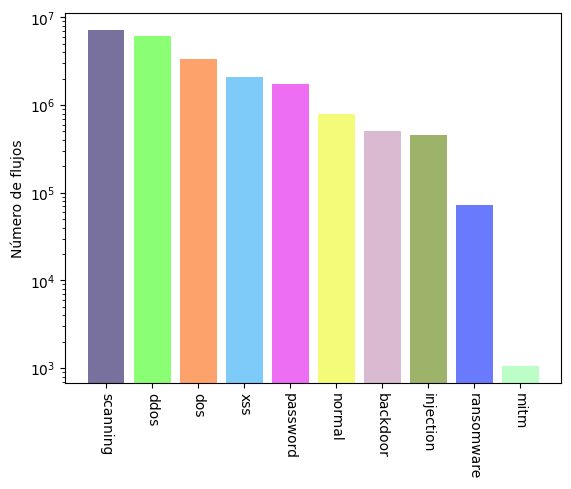
\includegraphics[width=0.49\linewidth]{media/toniot_csv_results.png}
  \end{center}
  \captionsetup{justification=centering}
  \caption{Distribución de ataques en TON-IoT}\label{fig:toniot_results}
\end{figure}

Si observamos la línea temporal de la figura \ref{fig:toniot_timeline} podemos ver ciertas tipologías de ataques distribuidos en el tiempo de maneras distintas. De todas maneras, a diferencia del caso de BoT-IoT los tamaños son comparables y se pueden mostrar en una misma escala. Los ataques de escaneo y puerta trasera son los que tienen mayor duración, a continuación tenemos los ataques de denegación de servicio distribuido, no distribuido e intentos de forzar las contraseñas. Finalmente, tenemos ataques de xss, inyección de datos y ransomware. Las cantidades de tráfico visto y sus extensiones temporales son relativamente consistentes con la tipología de ataque. Los ataques de mayor duración (escaneo y descubrimiento de contraseñas) se extienden durante el tiempo para tratar de pasar desapercibidos, los de denegación tratan de colapsar un servicio enviando mucho tráfico en poco tiempo y finalmente los ataques directos tienen una duración más restringida y son más directos. La excepción a esto último son los ataques de puerta trasera, que parecen extenderse en mayor medida a lo que cabria esperar. Es posible que esto sea debido a que la manera de realizar el ataque haya sido menos dirigida, tratando de encontrar una vulnerabilidad, probando diferentes opciones.

\begin{figure}[!htb]
  \begin{center}
      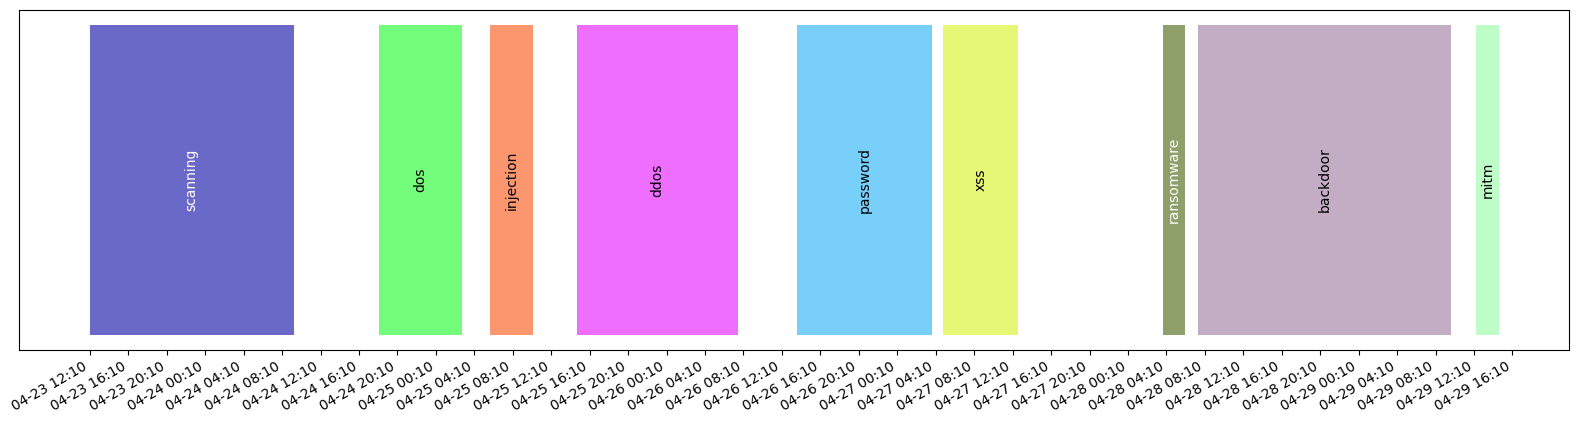
\includegraphics[width=1\linewidth]{media/toniot_csv_timeline.png}
  \end{center}
  \captionsetup{justification=centering}
  \caption{Línea temporal de las trazas con los tipos de ataque en Ton-Iot)}\label{fig:toniot_timeline}
\end{figure}

En total, hay 46 características disponibles en el dataset y explicadas en el conjunto de datos descargables. Manteniendo el formato, las características consisten en:

\begin{enumerate}
  \item \textbf{ts}: Tiempo de inicio del flujo expresado en tiempo Unix con segundos.
  \item \textbf{src\_ip}: Dirección IP de origen.
  \item \textbf{src\_port}: Puerto IP de origen.
  \item \textbf{dst\_ip}: Dirección IP de destino.
  \item \textbf{dst\_proto}: Puerto IP de destino.
  \item \textbf{proto}: Nombre del protocolo transporte utilizado.
  \item \textbf{service}: Protocolos de aplicación detectados, como DNS, HTTP y SSL.
  \item \textbf{duration}: Duración del flujo, calculado a partir de substraer el tiempo del último paquete detectado del primero.
  \item \textbf{src\_bytes}: Bytes enviados por el emisor inicial como datos sobre TCP, si aplica.
  \item \textbf{dst\_bytes}: Bytes enviados por el receptor inicial como datos sobre TCP, si aplica.
  \item \textbf{conn\_state}: Estado de la conexión, expresado como S0 (intento de conexión sin respuesta), S1 (conexión establecida) y REJ (conexión rechazada).
  \item \textbf{missed\_byttes}: Bytes perdidos detectados en la conexión TCP.
  \item \textbf{src\_pkts}: Número de paquetes enviados por el emisor inicial.
  \item \textbf{src\_ip\_bytes}: Número de bytes enviados sobre IP por el emisor inicial.
  \item \textbf{dst\_pkts}: Número de paquetes enviados por el receptor inicial.
  \item \textbf{dst\_ip\_bytes}: Número de bytes enviados sobre IP por el receptor inicial.
  \item \textbf{dns\_query}: Nombres pedidos en la petición DNS, si aplica.
  \item \textbf{dns\_qclass}: Entero indicando las clases de la petición DNS realizada, si aplica.
  \item \textbf{dns\_qtype}: Entero indicando los tipos de petición DNS realizada, si aplica.
  \item \textbf{dns\_rcode}: Entero indicando el código de respuesta del DNS, si aplica.
  \item \textbf{dns\_AA}: Indicador booleano si la respuesta del DNS es autoritativa, si aplica.
  \item \textbf{dns\_RD}: Indicador booleano si la petición DNS pide recursividad, si aplica.
  \item \textbf{dns\_RA}: Indicador booleano si el servidor DNS soporta recursividad, si aplica.
  \item \textbf{dns\_rejected}: Indicador booleano si el servidor DNS ha rechazado la petición, si aplica.
  \item \textbf{ssl\_version}: La versión SSL ofrecida por el servidor, si aplica
  \item \textbf{ssl\_cipher}: El conjunto de cifrados SSL escogido por el servidor, si aplica.
  \item \textbf{ssl\_resumed}: Indicador booleano indicando que la sesión SSL puede ser utilizada para generar conexiones, si aplica.
  \item \textbf{ssl\_established}: Indicador booleano indicando si existe una sesión SSL establecida, si aplica.
  \item \textbf{ssl\_subject}: Nombre del propietario del certificado SSL, si aplica.
  \item \textbf{ssl\_issuer}: Emisor del certificado SSL y autoridad, si aplica.
  \item \textbf{http\_trans\_depth}: Profundidad de la transferencia HTPP, si aplica.
  \item \textbf{http\_method}: Método HTTP utilizado, si aplica.
  \item \textbf{http\_uri}: URI utilizadas en la petición HTTP, si aplica.
  \item \textbf{http\_version}: Versión HTTP utilizada, si aplica.
  \item \textbf{http\_request\_body\_len}: Longitud de la petición HTTP, si aplica.
  \item \textbf{http\_response\_body\_len}: Longitud de la respuesta HTTP, si aplica.
  \item \textbf{http\_status\_code}: Codigo de respuesta de la petición HTTP, si aplica.
  \item \textbf{http\_user\_agent}: Valores del agente de usuario en la petición HTTP, si aplica.
  \item \textbf{http\_orig\_mime\_types}: Tipos de recursos pedidos en la petición HTTP, si aplica.
  \item \textbf{http\_resp\_mime\_types}: Tipos de recursos devueltos en la petición HTTP, si aplica.
  \item \textbf{weird\_name}: Nombres de las anomalías relacionadas con los protocolos ocurridos.
  \item \textbf{weird\_addl}: Información adicional asociada a las anomalías.
  \item \textbf{weird\_notice}: Indica si la anomalía se ha convertido en una notificación.
  \item \textbf{label}: Indicador si el flujo es normal (0) o un ataque (1)
  \item \textbf{type}: Nombre del tipo de flujo, siendo este normal o DoS, DDoS, etc.
\end{enumerate}

\subsubsection{Contenidos PCAPs}

El dataset TON-IoT ofrece 64 archivos (48.1 GiB) de trazas de red con tráfico normal y tráfico de  ataques entremezclados con tráfico normal. El tráfico sin ataques es alrededor de 15.6 GiB, un 32.43\% del total y el resto se encuentra repartido por cada tipo de ataque. El script utilizado para la extracción es \texttt{extract\_info\_toniot\_pcaps\_tshark.sh} y el utilizado para la representación de estos es \texttt{evaluate\_info\_toniot\_pcaps\_tshark.py} disponible en TODO DEFINIR.

En los PCAP, aparecen un total de 29 270 direcciones IP únicas, una cantidad mucho mayor que la que tenemos en los otros dos datasets. Aparte de las direcciones IP mencionadas explícitamente en el paper original, aparecen una dirección IP del posible router, la dirección IP de broadcast y 13 direcciones IP adicionales. Estas últimas son posiblemente los otros dispositivos IoT y dispositivos de usuarios, los cuales sus direcciones han sido asignadas por DHCP. Adicionalmente, hay 9 archivos, los cuales tshark ha notificado que tenían un corte en los datos.

% archivos pcap cortados 
%"/Datasets/TON-IoT/Raw_datasets/network_data/Network_dataset_pcaps/normal_attack_pcaps/Injection_normal/injection_normal1.pcap"
%"/Datasets/TON-IoT/Raw_datasets/network_data/Network_dataset_pcaps/normal_attack_pcaps/Injection_normal/injection_normal4.pcap" 
%"/Datasets/TON-IoT/Raw_datasets/network_data/Network_dataset_pcaps/normal_attack_pcaps/MITM_normal/MITM_normal2.pcap"
%"/Datasets/TON-IoT/Raw_datasets/network_data/Network_dataset_pcaps/normal_attack_pcaps/MITM_normal/MITM_normal3.pcap"
%"/Datasets/TON-IoT/Raw_datasets/network_data/Network_dataset_pcaps/normal_attack_pcaps/normal_DDoS/normal_DDoS_2.pcap"
%"/Datasets/TON-IoT/Raw_datasets/network_data/Network_dataset_pcaps/normal_attack_pcaps/normal_DoS/normal_DoS_1.pcap" 
%"/Datasets/TON-IoT/Raw_datasets/network_data/Network_dataset_pcaps/normal_attack_pcaps/password_normal/password_normal1.pcap"
%"/Datasets/TON-IoT/Raw_datasets/network_data/Network_dataset_pcaps/normal_pcaps/normal_IoT_2.pcap" 
%"/Datasets/TON-IoT/Raw_datasets/network_data/Network_dataset_pcaps/normal_pcaps/normal_IoT_3.pcap" 

Para este dataset, también se han generado diferentes histogramas para asegurar la consistencia de la herramienta. En este dataset, como podemos ver en la figura \ref{fig:toniot_pcap_duration_distribution}, los flujos se concentran principalmente en tiempos cortos y aparece una agrupación en el centro de la distribución y otra en las duraciones más elevadas. Sin embargo, los rangos son distintos, comparado con las figuras \ref{fig:cicddos_2019_pcap_duration_distribution} y \ref{fig:botiot_pcap_duration_distribution}. En las anteriores, el rango se comprendía entre 0 y 10 000 en el primer caso y 0 y 2000 en el segundo. En este, el rango es mucho más extenso, llegando hasta 100 000. Si miramos los números de tramas y bytes de las figuras \ref{fig:toniot_pcap_frames_distribution} y \ref{fig:toniot_pcap_bytes_distribution}, podemos ver que sigue una forma descendiente, con ciertos puntos más planos y algún pico. Esta distribución es distinta a la que nos hemos encontrado en BoT-IoT, donde había agrupaciones de tamaños, y de CIC-DDos2019, donde había un pico pronunciado al final del gráfico.

\begin{figure}[H]
  \begin{center}
      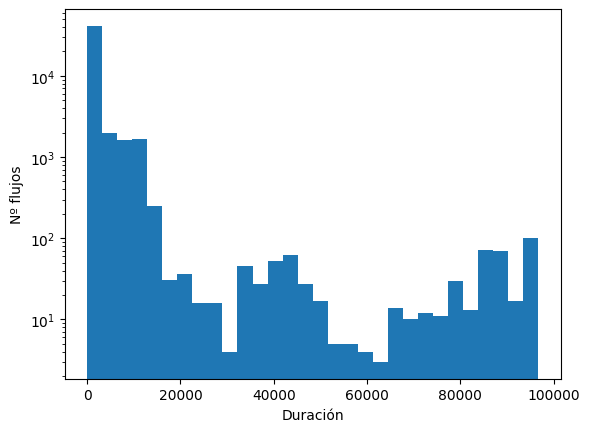
\includegraphics[width=0.49\linewidth]{media/toniot_pcap_duration_distribution.png}
  \end{center}
  \captionsetup{justification=centering}
  \caption{Distribución duraciones de flujos en TON-IoT}\label{fig:toniot_pcap_duration_distribution}
\end{figure}

\begin{figure}[H]
  \minipage{0.49\textwidth}
    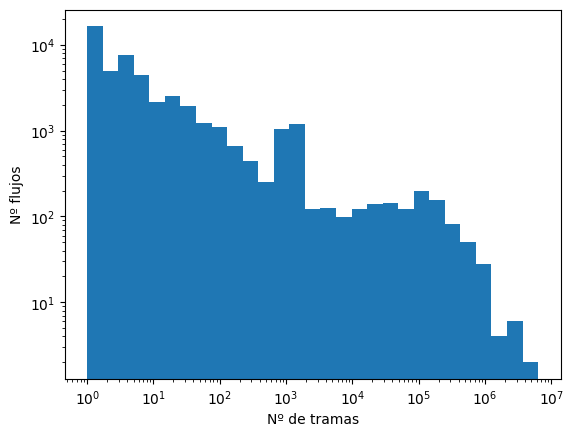
\includegraphics[width=\linewidth]{media/toniot_pcap_frames_distribution.png}
    \captionsetup{justification=centering}
    \caption{Distribución número de tramas en flujos en TON-IoT}\label{fig:toniot_pcap_frames_distribution}
  \endminipage\hfill
  \minipage{0.49\textwidth}
    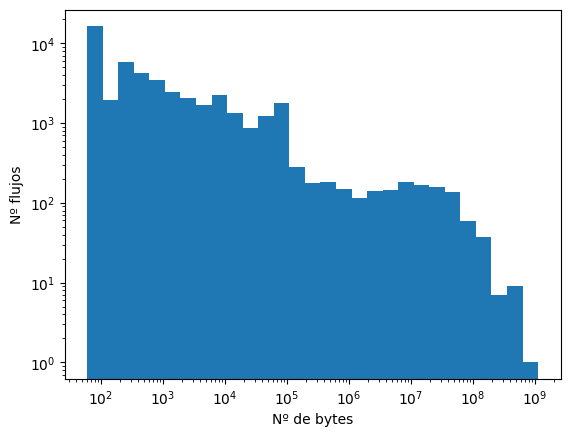
\includegraphics[width=\linewidth]{media/toniot_pcap_bytes_distribution.png}
    \captionsetup{justification=centering}
    \caption{Distribución número de bytes en flujos en TON-IoT}\label{fig:toniot_pcap_bytes_distribution}
  \endminipage\hfill
\end{figure}

En la tabla \ref{table:toniotprotocolsip} podemos ver el resultado del análisis con tshark sobre la repartición de los diferentes protocolos de transporte sobre IPv4. A diferencia de los otros casos, la mayoría de tramas en este dataset van sobre TCP (90.154\%) y tiene cierto tráfico que se puede considerar residual en UDP (5.982\%) y no identificado (3.864\%).

%Generated with /workspaces/tfg/scripts/evaluate_info_toniot_pcaps_tshark.py
\begin{table}[H]
    \begin{center}
        \begin{tabular}{|c | c c|} 
            \hline
            \textbf{Protocolo} & \textbf{Nº Tramas} & \textbf{Porcentaje}\\
            \hline\hline
IP & 1.92e+08 & 100.000 \\
TCP & 1.73e+08 & 90.154 \\
NONE & 7.40e+06 & 3.864 \\
UDP & 1.15e+07 & 5.982 \\
            \hline
        \end{tabular}
    \end{center}
    \caption{Protocolos identificados analizando exclusivamente la capa IP en TON-IoT}
    \label{table:toniotprotocolsip}
\end{table}


La tabla \ref{table:botiotprotocols}, que contiene las tres primeras capas de protocolos identificados en BoT-IoT, es de mayor tamaño que en los casos anteriores. Esto es debido a que aparece el uso de "sll" (no confundir con SSL) aparte del tráfico sobre Ethernet. Si abrimos los ficheros con WireShark, podemos observar que este consiste en el tipo "Linux cooked capture", el cual puede contener paquetes IP como en la figura \ref{fig:toniot_pcap_ssl_ip_packet} o paquetes Ethernet como en la figura \ref{fig:toniot_pcap_ssl_eth_packet}. Se puede observar en esta última que WireShark no es capaz de reconocer los contenidos de la siguiente capa. Esta capa de enlace no es una capa de enlace real, sino que es una especial para guardar trazas de red de forma más flexible. 

\begin{figure}[H]
  \minipage{0.49\textwidth}
  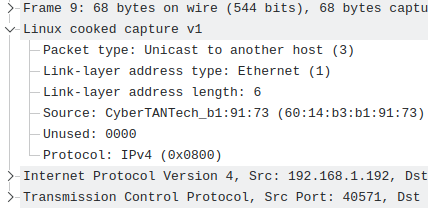
\includegraphics[width=\linewidth]{media/toniot_pcap_ssl_ip_packet.png}
  \captionsetup{justification=centering}
  \caption{Paquete SLL sin ETHII en TON-IOT}\label{fig:toniot_pcap_ssl_ip_packet}
  \endminipage\hfill
  \minipage{0.49\textwidth}
    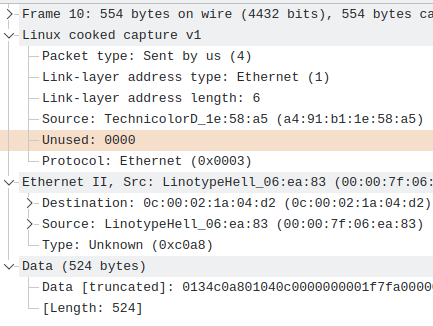
\includegraphics[width=\linewidth]{media/toniot_pcap_ssl_eth_packet.png}
    \captionsetup{justification=centering}
    \caption{Paquete SLL con EthII en TIN-IOT}\label{fig:toniot_pcap_ssl_eth_packet}
  \endminipage\hfill
\end{figure}

Podemos ver que la mayoría de los datos expresados en la tabla \ref{table:toniotprotocols} están encapsulados en SLL (34.4 GiB) y no se incluyen las cabeceras Ethernet originales, sino que aparece la capa IP directamente (22.8 GiB) y a continuación TCP (21.7 GiB). De todas maneras, hay una cantidad considerable de tramas (11.3 GiB), las cuales sí que incluyen la capa Ethernet. Adicionalmente, parte de los datos no utilizan SLL como encapsulación, sino que hacen uso de Ethernet como en los otros datasets (8.4 GiB). 

%Generated with /workspaces/tfg/scripts/evaluate_info_toniot_pcaps_tshark.py
\begin{table}[H]
    \begin{center}
        \begin{tabular}{|c c c | c c c|} 
            \hline
            \textbf{L0} & \textbf{L1} & \textbf{L2} & \textbf{Tramas} & \textbf{Bytes} & \textbf{Nº subprotocolos}\\
            \hline\hline
sll &- &- & 1.78e+08 & 34.3GiB & 4 \\
sll &ip &- & 1.55e+08 & 22.8GiB & 5 \\
sll &ip &tcp & 1.43e+08 & 21.7GiB & 36 \\
sll &ip &udp & 4.50e+06 & 498.0MiB & 46 \\
sll &ip &icmp & 7.51e+06 & 638.3MiB & 39 \\
sll &ip &data & 6.19e+02 & 909.5KiB & 0 \\
sll &ip &igmp & 4.78e+04 & 2.8MiB & 0 \\
sll &arp &- & 1.68e+06 & 98.1MiB & 1 \\
sll &arp &text & 1.57e+05 & 9.3MiB & 1 \\
sll &eth &- & 2.15e+07 & 11.3GiB & 1 \\
sll &eth &data & 2.15e+07 & 11.3GiB & 0 \\
sll &ipv6 &- & 1.26e+05 & 131.0MiB & 4 \\
sll &ipv6 &icmpv6 & 6.71e+04 & 5.6MiB & 1 \\
sll &ipv6 &udp & 1.04e+04 & 2.0MiB & 4 \\
sll &ipv6 &tcp & 4.80e+04 & 123.4MiB & 4 \\
sll &ipv6 &data & 1.00e+00 & 1.5KiB & 0 \\
eth &- &- & 3.72e+07 & 8.4GiB & 3 \\
eth &ip &- & 3.69e+07 & 8.4GiB & 5 \\
eth &ip &tcp & 2.66e+07 & 7.6GiB & 14 \\
eth &ip &udp & 6.80e+06 & 646.3MiB & 16 \\
eth &ip &data & 3.33e+02 & 492.3KiB & 0 \\
eth &ip &igmp & 5.02e+04 & 2.9MiB & 0 \\
eth &ip &icmp & 3.44e+06 & 205.5MiB & 3 \\
eth &arp &- & 2.52e+05 & 14.2MiB & 1 \\
eth &arp &text & 2.22e+04 & 1.3MiB & 1 \\
eth &ipv6 &- & 1.47e+04 & 3.3MiB & 3 \\
eth &ipv6 &icmpv6 & 7.03e+03 & 664.6KiB & 0 \\
eth &ipv6 &udp & 7.67e+03 & 2.7MiB & 6 \\
eth &ipv6 &tcp & 3.40e+01 & 3.1KiB & 0 \\
            \hline
        \end{tabular}
    \end{center}
    \caption{Primeras tres capas de protocolos identificados en TON-IoT}
    \label{table:toniotprotocols}
\end{table}

